\section{Title: Assessing Discrimination against Women and Underrepresented Minorities in Engineering and the Protective Impacts of Micro-climates}
\section{Introduction}
\label{sec:intro}

 
Engineering is a challenging discipline to study, made more so for students from groups traditionally underrepresented in the field who deal with discrimination, bias, microaggressions, and “othering” during their careers.
These groups include racial and ethnic minorities (\eg \cite{Mcgee:2011}), women (\eg \cite{Moss-Racusin:2012}), LGBTQIA+ identifying students (\eg \cite{Cech:2011}) and first-generation college students (\eg \cite{Pascarella:2004,carrigan2015onramping}.
Challenges can be compounded when multiple identities come into play (\eg \citep{Williams:2014}).
Despite significant funding and attention paid to diversity in engineering, the percentage of B.S. degrees awarded to women engineers in 2017 has increased by just 3\% over 2008 numbers, from 18\% to 21\% \citep{yoder2012engineering}. 
%\sandy{Couldn't this be (mis)interpreted as 'moving in the right direction'?}\jen{better?}
 
The choice to stay in engineering is complex, and there are many potential influences. However, one barrier in particular represents an unnecessary waste of talent and interest when it discourages students and minimizes their impact: Discrimination. Discrimination is defined as differential treatment or disparate impact of institutionalized processes that influences individuals or groups of people \citep{Pager:2008}. It is different from but can be caused by prejudice, stereotypes, and ideologies such as racism or sexism. Discriminatory encounters are ubiquitous, occurring in varied contexts from social interactions with peers, to workplace environments, to stores, to encounters with law enforcement, and of course in educational settings \cite{Fisher:2000}. Experiences of discrimination are undeniably consequential for the life trajectory of young people, particularly students. For example, discrimination, bias, micro-aggressions, and other forms of ``othering'' discourage many minorities from pursuing education in fields that are dominated by the privileged majority (\eg \cite{robinson2015racial}), such as STEM (Science, Technology, Engineering, and Mathematics). For students who do stay in their field, discrimination may directly impact success in the field as well as career prospects. For example, \citet{Moss-Racusin:2012} show that students' resumes with randomly assigned male names are rated as more competent, hireable, and worthy of more mentoring and pay than those same resumes when they are randomly assigned a female name. Relatedly, \citet{Williams:2010} present empirical evidence for salary estimation bias that can lead to employers offering lower pay to women workers who themselves are less likely to negotiate for equal pay. 

There are also long-term negative health consequences of exposure to discrimination and the stress it produces. For instance, heightened blood pressure, heart rate, and cortisol secretions, as markers of heart disease \cite{Marshall:1997, Cohen:1994}, have been reported in relation to perceived racism \cite{Brondolo:2008, Steffen:2003, Smart:2010}. There is also considerable evidence for the harmful effects of discrimination on mental health \cite{Pascoe:2009}. For example, \citet{Kessler:1999} report major depression, generalized anxiety disorders, and psychological distress associated with lifetime discrimination that are comparable in magnitude to those of major life events such as sexual assault. Day-to-day experiences of micro-aggressions, subtle forms of discrimination, are similarly deleterious to health as expressed by \cite{Solorzano:2000} and empirically supported by \cite{Ong:2009}. 

Thus, \textbf{there is unique potential for significant societal impact if we better understand how young adults experience discrimination.} If we can concretely quantify discrimination not only in terms of its prevalence but also in terms of its short-term impact on health and behavior, then we can better reason about pathways that connect the short-term impact to long-term outcome disparities that we currently observe in the population. 

\textbf{However, it has been difficult to effectively measure the day-to-day impact of discrimination.} Past research examining short-term influence of exposure to discrimination is mostly qualitative in nature (\eg \cite{Swim:2003} and \cite{Solorzano:2000}), and includes only a small number of self-reported measures in the context of diary studies that last only a few weeks (\eg \cite{Ong:2009}). These self-reported accounts are usually retrospective and therefore limited in their accuracy and comprehensiveness. Moreover, they lack details about changes at the behavioral level, which are sometimes subconscious and thus impossible to report. Knowledge about these behavioral changes is critical in identifying mechanisms that explain the impact of discrimination encounters. 

We strongly believe that a far more comprehensive approach to data collection is needed. In this era of digitally instrumented living, a comprehensive change in how we collect and assess data about the college student experience is possible. We can now connect self-reported experience to short-term changes in passively sensed behavior and to longitudinal outcomes. This, rich data in turn, makes it possible to understand bias in  new ways.  

%We now have the technological innovations needed to make this connection possible because we can access devices that passively capture many student activities.
A 2014 study demonstrates that large-scale, longitudinal data collection can facilitate our understanding of depression and other mental health factors and how they relate to student outcomes (\eg \cite{wang2014studentlife}). That study depended on occasional survey questions combined with a large amount of passive data collection. By complementing self reports with passive data collection, we can similarly use big data to create an image of behavior while learning about negative events underrepresented minority engineering students are exposed to. This ability to connect behavior to experience, in the field, was lacking in past studies. Ours is an exciting era for data collection and analysis, one where it is possible to study issues such as discrimination, bias and related adversity exposure at scale and in real-time to understand their various impacts. This important information will help support the design of effective interventions, policies, and decision making to improve the experiences of not just diverse students in engineering, but of all students in engineering. 
 
These insights led us to raise seed money to launch a pilot study with 200 students in 2018. Since then, we have revised our study protocol to further improve it, completed an initial analysis we discuss in this proposal, and begun year one of data collection with a new cohort of 200 first-year students. In both the pilot study and year one, we ensured inclusion of a representative sample of underrepresented groups in engineering (UREs), as shown in Table~\ref{tab:study-participants}. This includes women, underrepresented minorities, first-generation college students, and LGBTQ students. While we are still collecting year one data as of this writing, our pilot data showed high compliance and the significance of the rich, varied data we collected for understanding discrimination.

Ninety-one participants from the pilot reported  454 separate instances of discrimination, and we demonstrated the impact of these experiences on their sleep and phone use and connected these behaviors to emotional state.  
We propose to follow as many of the 200 students from year one as possible for an additional three years to fully understand the longitudinal impact of discrimination on engineering students’ experiences and success. While the data from year one reveal short-term impacts of discrimination, additional data will confirm our observations thus far and shed more needed light on critical long-term impacts, such as retention.

%\paula{below the term challenges is used. This is fine but we will need to think about wording consistency. I used adversity exposure above and we use negative events later. At some points we will be pulling from our fuller data such as MLEs, poverty, ACEs, etc as part of a broader stress assessment within which discrimination is embedded. }

\subsection{Intellectual Merit}
\label{sec:questions}

Our proposed work will leverage the data collected thus far to improve our theoretical understanding of the impact of discrimination on students; answer important questions about both short- and long-term impacts of discrimination; illuminate mediating factors, such as other forms of adversity exposure and resilience as well as influences of micro-climates; and ultimately support intervention design.
%\paula{I revised above as the figure does not portray micro-climates in a mediating role but seems more related to capturing nuances of key micro-climates.}
We  propose to test a model of the student experience (shown in Figure~\ref{fig:model}) that we believe helps capture the differential stressors experienced by women and minorities in engineering in a way that can ultimately be quantified and operationalized. 

%\jen{add discussion of rich ema and behavioral data; possibly add interviews; sample size: can we argue for a larger survey? Or for big data within people? methodological solutions? How do we address stability and analysis. rich small data rather than big data}

As shown in Figure~\ref{fig:model} and described in more depth in Section~\ref{sec:back}, much is known about the relationship between the overall stress burden faced by students from different backgrounds, discrimination and long-term stress outcomes, such as physical and mental health \paula{I don't know if more refs are useful but \citet{Pascoe:2009} offer a meta-analysis and similar model that may be worth a look. I have the pdf} (\eg \cite{Ong:2009}). However, many open questions remain, which will constitute the focus of our work; these are shown in Figure~\ref{fig:model} in the boxes with dashed lines along the dashed arrows. We intend to answer four primary questions. Here, we discuss and explain the importance of each.

\begin{figure}
    \centering
    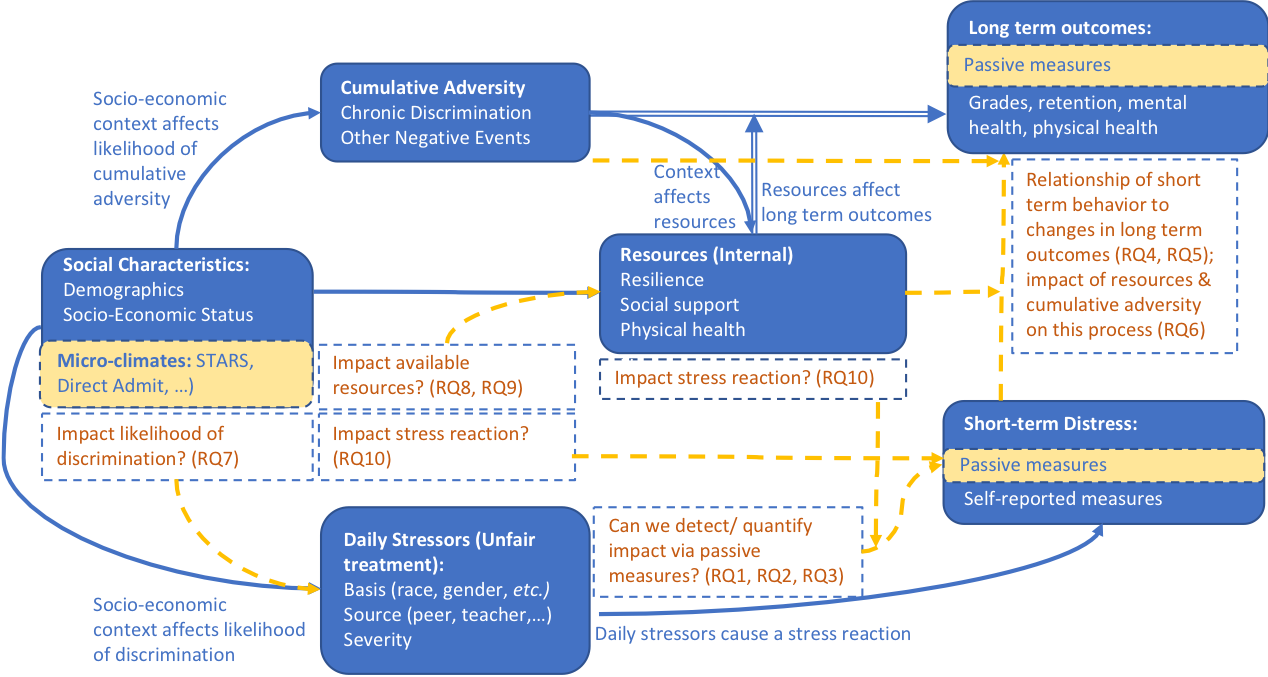
\includegraphics[width=14cm]{img/discrimination-model.png}
    \caption{Theoretical model relating student experiences to long-term outcomes.}
    \label{fig:model}
\end{figure}


\paragraph{Daily Discrimination $\rightarrow$ Short-Term Behavior} Our pilot study already revealed almost 450 separate instances of  \textit{daily discrimination} together with extensive passively-collected behavioral data, unlike any former study. Thus, our first research questions ask what we can learn about the impact of daily discrimination from behavioral data. This is particularly important in an educational context, where we may find, for example, that discrimination is both more likely at high-stress times (such as midterms) and more impactful at these times (if students lose sleep and are thus less well prepared). 
\begin{enumerate}[start=1,label={\bfseries RQ\arabic*}, leftmargin=1cm]
    \item \label{itm:rq-behavior} What is the impact of daily discrimination on short-term behaviors? \paula{the model suggests to me that this question also encompasses effects of the mediating factors. That any given discriminatory event does not carry "pure" effect. Do we want to "set up" in intro analysis re consideration of effects of mediating variables in conjunction with discrimination? If that seems confusing or problematic, cool. if we'd like to consider other analytic approaches, such as \cite{Ong:2009} \textit{et al's} attention to negative effects, am happy to discuss. } We hypothesize that this impact is similar to that for stress, which leads to the following question.
    \item \label{itm:rq-behavior-size} Can we quantify both the scope of any behavior change due to a daily discrimination event, and the length of time it is likely to persist? 
    \item \label{itm:rq-severity-impact} Does the severity of the discrimination event(s) change these outcomes?
\end{enumerate}

\paragraph{Short-Term Behavior $\rightarrow$ Long-Term Outcomes} Our second set of questions follows from the first by extending findings to a longitudinal data set. While the impact of discrimination on long-term outcomes has been studied, no prior data set has been able to relate both short- and long-term impacts as we intend to do. \eve{say more about how LT and ST relate}
\begin{enumerate}[start=4,label={\bfseries RQ\arabic*}, leftmargin=1cm]
    \item \label{itm:rq-short-long} Which long-term outcomes are linked to short-term behavior changes, and to what degree? \sandy{Note that many of these questions make assumptions, e.g., that long-term outcomes ARE linked to s-t behavior changes.  Should you ask the question, "Are long-term outcomes linked to short-term behavior changes? How, and to what degree?}
    \item \label{itm:rq-which-long} Are some short-term changes more likely to relate to long-term impacts than others? \paula{We may not want to pursue it, but the model illustrates the capacity to assess daily discrimination and mediating factors as co-contributors to long term impacts. I am finding myself unclear how to think about short term behaviors as major contributors aside from stressors as key contributors to long term behavior and well being}
    \item \label{itm:rq-severity-long} Do specific factors, such as cumulative impact of discrimination or number of repetitions, predict long-term impacts? \paula[again, do we want to frame this as looking at cumulative discrim in conjuction with chronic discrim and other adversities or negative events?]
\end{enumerate}
 
\begin{WrapText}
\begin{description}[leftmargin=1cm]
\item[STARS] The Washington State Academic RedShirt (STARS) program supports engineering and computer science students from low-income, first-generation, and underserved backgrounds in navigating the transition to college.
STARS is a two-year program with a specialized curriculum designed to build learning skills and strengthen academic preparation for core math and science prerequisites. STARS scholars are guaranteed placement into an engineering or computer science major.

\item[Introductory Sequence] The introductory course experience can significantly affect the likelihood of discrimination due to the level of competitiveness...
\item[SEEEDS Bridge Program] Through the Summer Early Enrichment in Engineering for Dean's Scholars (SEEEDS), incoming first-year engineering students get support to succeed in their first prerequisite courses at UW.  They also build community and learn about the myriad academic and professional development resources for UW students. 
\item[FIGS?]
\end{description}
\end{WrapText}

 \paragraph{Micro-Climates $\rightarrow$ Indirect Impact} Although novel intervention design is beyond the scope of this proposal, we intend for the proposed work to clarify the impact of existing micro-climates, which can in turn guide intervention design. We have already identified multiple micro-climates that could affect the discrimination-stress process highlighted in Figure~\ref{fig:model}, including the Washington \textbf{St}ate \textbf{A}cademic \textbf{R}ed\textbf{S}hirt (STARS) program; introductory course sequences that students must take; and participation in the Summer Early Enrichment for Engineering for Dean's Scholars (SEEEDS) bridge program (see Sidebar~\ref{sidebar:definitions}). \paula{useful to define earlier or here what micro-climates are defined as? \sandy{Yes, please define this term.} how will negative micro-climates or those beyond the noted groups be assessed? do settings like labs or other routine places respondents spend time considered micro-climates?} We believe that these micro-climates will indirectly affect outcomes through their impact on mediating factors and the likelihood of daily discrimination events. \eve{what are mediating factors? What do we mean by their impact}\jen{we probably need to decide whether to say mediating or moderating. Could be a question for Paula}
 
\begin{enumerate}[start=7,label={\bfseries RQ\arabic*}, leftmargin=1cm]
    \item \label{itm:mc-daily-discrimination} Which micro-climates will reduce exposure to daily discrimination? Which micro-climates will increase exposure?\sandy{Again, rephrase:  Will micro-climates reduce/increase exposure to daily discrimination?}

    \item \label{itm:mc-external-mediators} Which micro-climates will increase or decrease external mediating factors, such as exposure to negative events? Will this translate into different short- or long-term behavioral outcomes using the mechanisms identified in the prior RQs?
    \item \label{itm:mc-internal-mediators} Which micro-climates will increase or decrease internal mediating factors, such as resilience and two-way social support? Will this translate into different short- or long-term behavior outcomes using the mechanisms identified in the prior RQs?
    \item \label{itm:mc-mediators-behavior} How important are mediating factors to short term behaviors (to what extent to they cause responses to be much larger or smaller?). How does this impact the translation of short term behavior into long term outcomes?
\end{enumerate}
 
We seek to develop a holistic understanding of the impacts of discrimination on the participation and retention of UREs throughout  their college career. Specific contributions of our work will include: (1) a \textbf{more complete theoretical model} of the impact of discrimination than those provided in previous work.  Our research will also make it possible: (2) to document, for the first time, \textbf{what behaviors change and in what ways} following acts of discrimination, and (3) to demonstrate, for the first time, \textbf{which micro-climates reduce that impact and through what mechanisms}. Finally, this in turn can (4) guide the \textbf{development of interventions }that help to mediate or reduce the experience of discrimination.  

\subsection{Broader Impact}
\noindent
Our proposed work will improve outcomes for UREs by: (1) \textbf{quantifying impact of unfair treatment} (i.e., discrimination, harassment, etc.)  on students; (2) \textbf{demonstrating to what degree discrimination impacts the success and retention} of underserved groups; and (3) \textbf{quantifying the protective impact of a currently deployed intervention}, an intentionally created micro-climate targeted at the most under-prepared  students in Engineering and Computer Science. 

The University of Washington is one of 8 or 10 large flagship public universities in the country. \sandy{hmmm, it's not in top 10 in terms of enrollment - https://www.stilt.com/blog/2018/01/americas-10-largest-universities-enrollment/.  What does "flagship" mean here?} Student experiences in different university settings are likely to be similar in terms of program scale and the range of students and student backgrounds entering the engineering program. This makes it likely that similar interventions will work in similar ways. The impact of discrimination on mental and physical health is already well-demonstrated in multiple studies. Thus, we expect that our findings will translate to similar large public universities, meaning that we have the potential to impact X 1000 engineers in training each year. We believe that our work will translate to engineering programs at other universities that are working to increase their diversity, as well. 

To this end, we will disseminate the results of our proposed research to other universities working to retain underserved students in Engineering and Computer Science.  Co-PI Riskin is PI of the UW STARS program, which was founded at UW and Washington State University in 2013;  STARS is an adaptation of the Goldshirt Program at the University of Colorado, Boulder, now entering its 11th year. Through UW’s leadership, the 'redshirt' model has since been adopted at three additional institutions through a six-institution Redshirt in Engineering Consortium grant from the National Science Foundation (UW, WSU, University of Colorado, Boulder, University of Illinois, Urbana-Champaign, Boise State University, and University of California, San Diego). Through the Redshirt Consortium, UW is engaged in sharing best practices to support first-generation students and those from low-income backgrounds. 

In the remainder of this proposal, we describe the pilot study that we have already conducted. We also present a simple, preliminary analysis of our data, which demonstrates the promise that our approach can indeed support investigation of our important research questions R1-R9.
 
\subsection{Team}
 
Jennifer Mankoff is the Richard E. Ladner professor in the Paul G. Allen School of Computer Science and Engineering. She has worked with underrepresented populations for over a decade (\eg \cite{newman2004perceptions,DBLP:conf/huc/DillahuntMPF09,DBLP:conf/cscw/DillahuntM14,DBLP:conf/huc/DillahuntMP10,DBLP:journals/pacmhci/EarlyHHRWM18,DBLP:conf/chi/OLearyZMR19}). In addition, she has led this study effort at the University of Washington (UW), helped to build the research team, and will continue to lead the effort over the remaining years of the study. Her background in Human Computer Interaction has prepared her well to conduct research of this scope, and her research includes a mix of qualitative behavioral work (\eg \cite{DBLP:conf/huc/DillahuntMPF09,DBLP:conf/chi/MankoffKKRW11}), mixed-methods/quantitative behavioral work (\eg \cite{DBLP:conf/ph/CrawfordGSAM14,DBLP:journals/pacmhci/EarlyHHRWM18}) and technical work in behavior modeling (\eg \cite{DBLP:conf/chi/BanovicBCMD16}). 
 
Eve Riskin is Professor of Electrical and Computer Engineering, Associate Dean of Diversity \& Access in the UW College of Engineering, and founder of the UW STARS program. As Faculty Director of UW's ADVANCE program, she has been working to promote diversity and inclusion in engineering for nearly two decades and has published extensively in this area (EVE-FILL-IN-HERE ).
 
Paula Nurius is the Grace Beals Ferguson Professor and Associate Dean at the UW School of Social Work. She brings many years of research and training experience in the areas of stress processes and short-term and life-course effects of discrimination, cumulative adversity and social disadvantage among both general and at-risk populations, including students. Prominent outcomes address mental and physical health, school experiences, and prevention and intervention implications (IF CITES NEEDED I CAN PROVIDE SOME). Her background in relevant social science theories, measures, and analytic strategies complements the expertise of other team members. 
